\chapter{Einleitung}
\label{cha:Einleitung}

\section{Problemstellung}
Eine sehr zentrale Eigenschaft von Software ist die Tatsache, dass immer wieder Änderungen stattfinden. Durch die Entwicklung, welche meist über lange Zeit von verschiedenen Programmierern oder Programmiererinnen vorgenommen wird, ergibt sich meist ein sehr unlesbarer, schwer zu wartender und schwer zu testender Code.
Diese Probleme führen in weitere Folge zu Qualitätseinbußen, da durch die schlechte Testbarkeit schlichtweg auf wichtige Tests verzichtet wird, da die Zeit für
die Implementierung dieser zu lange dauern würde. Eine weitere Folge der schlechten Lesbarkeit, ist die sich daraus ergebenden Schwierigkeiten beim Ändern des vorhandenen Codes. Dieser lässt sich nämlich nur noch unter sehr großem Aufwand und sehr großem Risiko, da er meist auch nicht durch Tests abgedeckt ist ändern,
was wiederum dazu führt, dass weniger Änderungen vorgenommen werden. Im schlimmsten Fall führen diese Probleme schlussendlich zum Scheitern des Projektes und es 
muss eingestellt werden, da der Aufwand der nötig wäre neue Änderungen oder Fehlerbehebungen vorzunehmen zu groß wäre. 

\section{Motivation}
In der modernen Softwareentwicklung geht es in erster Linie um das Umsetzen funktionaler sowie nicht funktionaler
Anforderungen und um die Behebung von Fehlern welche bei der Umsetzung dieser Anforderungen häufig auftreten. Ein wichtiger Punkt dabei ist, den Code so zu gestalten, dass er nicht nur vom Programmierer, der ihn geschrieben hat, gelesen werden kann, sondern auch von anderen Programmieren und dies auch möglichst noch nach mehreren Monaten. Um dies zu erreichen, müssen gewisse Grundsätze angewendet werden. In den letzten Jahren hat sich zu diesem Thema eine Strömung ergeben welche sich als Clean Code Development (im folgenden nur noch als CCD abgekürzt) bezeichnet. Geprägt wurde diese Bewegung in erster Linie von Robert. C. Martin und seinem Bestseller Clean Coder. Umso genauer man darauf achtet, den Code beim Schreiben lesbar zu gestalten, umso leichter wird es diesen auch noch nach einiger Zeit wieder zu Lesen. Bei schlecht geschrieben Code kann es sein, dass man bereits nach einigen Tagen nicht mehr genau weiß, was man damit bezwecken wollte. 

\section{Lösungsvorschlag}
CCD bietet für diese Probleme eine Lösung, welche aber über mehrere Jahre hinweg in den Entwicklungsteams etabliert werden muss. Der wichtigsten Punkte in CCD sind die folgenden:

\begin{figure}[h]
	\centering
		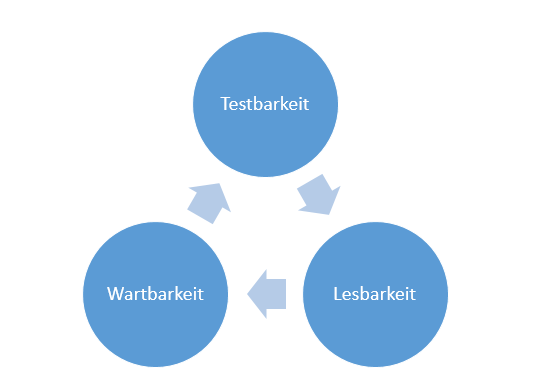
\includegraphics[width=1.00\textwidth]{images/cycle.PNG}
	\caption{CCD Zyklus}
	\label{fig:cycle}
\end{figure}

In der Abbildung \ref{fig:cycle} kann man gut erkennen, dass diese drei Hauptpunkte voneinander abhängen. Durch die gute Lesbarkeit, wird die Wartbarkeit des Codes erhöht da sich selbst ein neuer Mitarbeiter schnell einlesen kann und gut erkennen kann welche Aufgabe der aktuell betrachtete Code hat. Durch die bessere Wartbarkeit ergibt sich im weiteren auch die besseren Testbarkeit, welche für die Qualität der Software von hoher Bedeutung ist, da nur für getesteten Code sichergestellt werden kann, dass dieser auch wirklich die gewünschte Aufgabe richtig erledigt. Diese verbesserte Testbarkeit führt schließlich zu einer besseren Lesbarkeit, da die Test mit einer Dokumentation des Codes verglichen werden können. Sie zeigen welche Ausgabe erwartet werden kann und meist zeigen diese Tests auch Grenzfälle.

